
% Default to the notebook output style

    


% Inherit from the specified cell style.




    
\documentclass[11pt]{article}

    
    
    \usepackage[T1]{fontenc}
    % Nicer default font (+ math font) than Computer Modern for most use cases
    \usepackage{mathpazo}

    % Basic figure setup, for now with no caption control since it's done
    % automatically by Pandoc (which extracts ![](path) syntax from Markdown).
    \usepackage{graphicx}
    % We will generate all images so they have a width \maxwidth. This means
    % that they will get their normal width if they fit onto the page, but
    % are scaled down if they would overflow the margins.
    \makeatletter
    \def\maxwidth{\ifdim\Gin@nat@width>\linewidth\linewidth
    \else\Gin@nat@width\fi}
    \makeatother
    \let\Oldincludegraphics\includegraphics
    % Set max figure width to be 80% of text width, for now hardcoded.
    \renewcommand{\includegraphics}[1]{\Oldincludegraphics[width=.8\maxwidth]{#1}}
    % Ensure that by default, figures have no caption (until we provide a
    % proper Figure object with a Caption API and a way to capture that
    % in the conversion process - todo).
    \usepackage{caption}
    \DeclareCaptionLabelFormat{nolabel}{}
    \captionsetup{labelformat=nolabel}

    \usepackage{adjustbox} % Used to constrain images to a maximum size 
    \usepackage{xcolor} % Allow colors to be defined
    \usepackage{enumerate} % Needed for markdown enumerations to work
    \usepackage{geometry} % Used to adjust the document margins
    \usepackage{amsmath} % Equations
    \usepackage{amssymb} % Equations
    \usepackage{textcomp} % defines textquotesingle
    % Hack from http://tex.stackexchange.com/a/47451/13684:
    \AtBeginDocument{%
        \def\PYZsq{\textquotesingle}% Upright quotes in Pygmentized code
    }
    \usepackage{upquote} % Upright quotes for verbatim code
    \usepackage{eurosym} % defines \euro
    \usepackage[mathletters]{ucs} % Extended unicode (utf-8) support
    \usepackage[utf8x]{inputenc} % Allow utf-8 characters in the tex document
    \usepackage{fancyvrb} % verbatim replacement that allows latex
    \usepackage{grffile} % extends the file name processing of package graphics 
                         % to support a larger range 
    % The hyperref package gives us a pdf with properly built
    % internal navigation ('pdf bookmarks' for the table of contents,
    % internal cross-reference links, web links for URLs, etc.)
    \usepackage{hyperref}
    \usepackage{longtable} % longtable support required by pandoc >1.10
    \usepackage{booktabs}  % table support for pandoc > 1.12.2
    \usepackage[inline]{enumitem} % IRkernel/repr support (it uses the enumerate* environment)
    \usepackage[normalem]{ulem} % ulem is needed to support strikethroughs (\sout)
                                % normalem makes italics be italics, not underlines
    \usepackage{mathrsfs}
    

    
    
    % Colors for the hyperref package
    \definecolor{urlcolor}{rgb}{0,.145,.698}
    \definecolor{linkcolor}{rgb}{.71,0.21,0.01}
    \definecolor{citecolor}{rgb}{.12,.54,.11}

    % ANSI colors
    \definecolor{ansi-black}{HTML}{3E424D}
    \definecolor{ansi-black-intense}{HTML}{282C36}
    \definecolor{ansi-red}{HTML}{E75C58}
    \definecolor{ansi-red-intense}{HTML}{B22B31}
    \definecolor{ansi-green}{HTML}{00A250}
    \definecolor{ansi-green-intense}{HTML}{007427}
    \definecolor{ansi-yellow}{HTML}{DDB62B}
    \definecolor{ansi-yellow-intense}{HTML}{B27D12}
    \definecolor{ansi-blue}{HTML}{208FFB}
    \definecolor{ansi-blue-intense}{HTML}{0065CA}
    \definecolor{ansi-magenta}{HTML}{D160C4}
    \definecolor{ansi-magenta-intense}{HTML}{A03196}
    \definecolor{ansi-cyan}{HTML}{60C6C8}
    \definecolor{ansi-cyan-intense}{HTML}{258F8F}
    \definecolor{ansi-white}{HTML}{C5C1B4}
    \definecolor{ansi-white-intense}{HTML}{A1A6B2}
    \definecolor{ansi-default-inverse-fg}{HTML}{FFFFFF}
    \definecolor{ansi-default-inverse-bg}{HTML}{000000}

    % commands and environments needed by pandoc snippets
    % extracted from the output of `pandoc -s`
    \providecommand{\tightlist}{%
      \setlength{\itemsep}{0pt}\setlength{\parskip}{0pt}}
    \DefineVerbatimEnvironment{Highlighting}{Verbatim}{commandchars=\\\{\}}
    % Add ',fontsize=\small' for more characters per line
    \newenvironment{Shaded}{}{}
    \newcommand{\KeywordTok}[1]{\textcolor[rgb]{0.00,0.44,0.13}{\textbf{{#1}}}}
    \newcommand{\DataTypeTok}[1]{\textcolor[rgb]{0.56,0.13,0.00}{{#1}}}
    \newcommand{\DecValTok}[1]{\textcolor[rgb]{0.25,0.63,0.44}{{#1}}}
    \newcommand{\BaseNTok}[1]{\textcolor[rgb]{0.25,0.63,0.44}{{#1}}}
    \newcommand{\FloatTok}[1]{\textcolor[rgb]{0.25,0.63,0.44}{{#1}}}
    \newcommand{\CharTok}[1]{\textcolor[rgb]{0.25,0.44,0.63}{{#1}}}
    \newcommand{\StringTok}[1]{\textcolor[rgb]{0.25,0.44,0.63}{{#1}}}
    \newcommand{\CommentTok}[1]{\textcolor[rgb]{0.38,0.63,0.69}{\textit{{#1}}}}
    \newcommand{\OtherTok}[1]{\textcolor[rgb]{0.00,0.44,0.13}{{#1}}}
    \newcommand{\AlertTok}[1]{\textcolor[rgb]{1.00,0.00,0.00}{\textbf{{#1}}}}
    \newcommand{\FunctionTok}[1]{\textcolor[rgb]{0.02,0.16,0.49}{{#1}}}
    \newcommand{\RegionMarkerTok}[1]{{#1}}
    \newcommand{\ErrorTok}[1]{\textcolor[rgb]{1.00,0.00,0.00}{\textbf{{#1}}}}
    \newcommand{\NormalTok}[1]{{#1}}
    
    % Additional commands for more recent versions of Pandoc
    \newcommand{\ConstantTok}[1]{\textcolor[rgb]{0.53,0.00,0.00}{{#1}}}
    \newcommand{\SpecialCharTok}[1]{\textcolor[rgb]{0.25,0.44,0.63}{{#1}}}
    \newcommand{\VerbatimStringTok}[1]{\textcolor[rgb]{0.25,0.44,0.63}{{#1}}}
    \newcommand{\SpecialStringTok}[1]{\textcolor[rgb]{0.73,0.40,0.53}{{#1}}}
    \newcommand{\ImportTok}[1]{{#1}}
    \newcommand{\DocumentationTok}[1]{\textcolor[rgb]{0.73,0.13,0.13}{\textit{{#1}}}}
    \newcommand{\AnnotationTok}[1]{\textcolor[rgb]{0.38,0.63,0.69}{\textbf{\textit{{#1}}}}}
    \newcommand{\CommentVarTok}[1]{\textcolor[rgb]{0.38,0.63,0.69}{\textbf{\textit{{#1}}}}}
    \newcommand{\VariableTok}[1]{\textcolor[rgb]{0.10,0.09,0.49}{{#1}}}
    \newcommand{\ControlFlowTok}[1]{\textcolor[rgb]{0.00,0.44,0.13}{\textbf{{#1}}}}
    \newcommand{\OperatorTok}[1]{\textcolor[rgb]{0.40,0.40,0.40}{{#1}}}
    \newcommand{\BuiltInTok}[1]{{#1}}
    \newcommand{\ExtensionTok}[1]{{#1}}
    \newcommand{\PreprocessorTok}[1]{\textcolor[rgb]{0.74,0.48,0.00}{{#1}}}
    \newcommand{\AttributeTok}[1]{\textcolor[rgb]{0.49,0.56,0.16}{{#1}}}
    \newcommand{\InformationTok}[1]{\textcolor[rgb]{0.38,0.63,0.69}{\textbf{\textit{{#1}}}}}
    \newcommand{\WarningTok}[1]{\textcolor[rgb]{0.38,0.63,0.69}{\textbf{\textit{{#1}}}}}
    
    
    % Define a nice break command that doesn't care if a line doesn't already
    % exist.
    \def\br{\hspace*{\fill} \\* }
    % Math Jax compatibility definitions
    \def\gt{>}
    \def\lt{<}
    \let\Oldtex\TeX
    \let\Oldlatex\LaTeX
    \renewcommand{\TeX}{\textrm{\Oldtex}}
    \renewcommand{\LaTeX}{\textrm{\Oldlatex}}
    % Document parameters
    % Document title
    \title{Introduction to Python - Lesson 2}
    \author{Matteo Sani \\ \href{mailto:matteosan1@gmail.com}{matteosan1@gmail.com}}
   
    
    
    

    % Pygments definitions
    
\makeatletter
\def\PY@reset{\let\PY@it=\relax \let\PY@bf=\relax%
    \let\PY@ul=\relax \let\PY@tc=\relax%
    \let\PY@bc=\relax \let\PY@ff=\relax}
\def\PY@tok#1{\csname PY@tok@#1\endcsname}
\def\PY@toks#1+{\ifx\relax#1\empty\else%
    \PY@tok{#1}\expandafter\PY@toks\fi}
\def\PY@do#1{\PY@bc{\PY@tc{\PY@ul{%
    \PY@it{\PY@bf{\PY@ff{#1}}}}}}}
\def\PY#1#2{\PY@reset\PY@toks#1+\relax+\PY@do{#2}}

\expandafter\def\csname PY@tok@w\endcsname{\def\PY@tc##1{\textcolor[rgb]{0.73,0.73,0.73}{##1}}}
\expandafter\def\csname PY@tok@c\endcsname{\let\PY@it=\textit\def\PY@tc##1{\textcolor[rgb]{0.25,0.50,0.50}{##1}}}
\expandafter\def\csname PY@tok@cp\endcsname{\def\PY@tc##1{\textcolor[rgb]{0.74,0.48,0.00}{##1}}}
\expandafter\def\csname PY@tok@k\endcsname{\let\PY@bf=\textbf\def\PY@tc##1{\textcolor[rgb]{0.00,0.50,0.00}{##1}}}
\expandafter\def\csname PY@tok@kp\endcsname{\def\PY@tc##1{\textcolor[rgb]{0.00,0.50,0.00}{##1}}}
\expandafter\def\csname PY@tok@kt\endcsname{\def\PY@tc##1{\textcolor[rgb]{0.69,0.00,0.25}{##1}}}
\expandafter\def\csname PY@tok@o\endcsname{\def\PY@tc##1{\textcolor[rgb]{0.40,0.40,0.40}{##1}}}
\expandafter\def\csname PY@tok@ow\endcsname{\let\PY@bf=\textbf\def\PY@tc##1{\textcolor[rgb]{0.67,0.13,1.00}{##1}}}
\expandafter\def\csname PY@tok@nb\endcsname{\def\PY@tc##1{\textcolor[rgb]{0.00,0.50,0.00}{##1}}}
\expandafter\def\csname PY@tok@nf\endcsname{\def\PY@tc##1{\textcolor[rgb]{0.00,0.00,1.00}{##1}}}
\expandafter\def\csname PY@tok@nc\endcsname{\let\PY@bf=\textbf\def\PY@tc##1{\textcolor[rgb]{0.00,0.00,1.00}{##1}}}
\expandafter\def\csname PY@tok@nn\endcsname{\let\PY@bf=\textbf\def\PY@tc##1{\textcolor[rgb]{0.00,0.00,1.00}{##1}}}
\expandafter\def\csname PY@tok@ne\endcsname{\let\PY@bf=\textbf\def\PY@tc##1{\textcolor[rgb]{0.82,0.25,0.23}{##1}}}
\expandafter\def\csname PY@tok@nv\endcsname{\def\PY@tc##1{\textcolor[rgb]{0.10,0.09,0.49}{##1}}}
\expandafter\def\csname PY@tok@no\endcsname{\def\PY@tc##1{\textcolor[rgb]{0.53,0.00,0.00}{##1}}}
\expandafter\def\csname PY@tok@nl\endcsname{\def\PY@tc##1{\textcolor[rgb]{0.63,0.63,0.00}{##1}}}
\expandafter\def\csname PY@tok@ni\endcsname{\let\PY@bf=\textbf\def\PY@tc##1{\textcolor[rgb]{0.60,0.60,0.60}{##1}}}
\expandafter\def\csname PY@tok@na\endcsname{\def\PY@tc##1{\textcolor[rgb]{0.49,0.56,0.16}{##1}}}
\expandafter\def\csname PY@tok@nt\endcsname{\let\PY@bf=\textbf\def\PY@tc##1{\textcolor[rgb]{0.00,0.50,0.00}{##1}}}
\expandafter\def\csname PY@tok@nd\endcsname{\def\PY@tc##1{\textcolor[rgb]{0.67,0.13,1.00}{##1}}}
\expandafter\def\csname PY@tok@s\endcsname{\def\PY@tc##1{\textcolor[rgb]{0.73,0.13,0.13}{##1}}}
\expandafter\def\csname PY@tok@sd\endcsname{\let\PY@it=\textit\def\PY@tc##1{\textcolor[rgb]{0.73,0.13,0.13}{##1}}}
\expandafter\def\csname PY@tok@si\endcsname{\let\PY@bf=\textbf\def\PY@tc##1{\textcolor[rgb]{0.73,0.40,0.53}{##1}}}
\expandafter\def\csname PY@tok@se\endcsname{\let\PY@bf=\textbf\def\PY@tc##1{\textcolor[rgb]{0.73,0.40,0.13}{##1}}}
\expandafter\def\csname PY@tok@sr\endcsname{\def\PY@tc##1{\textcolor[rgb]{0.73,0.40,0.53}{##1}}}
\expandafter\def\csname PY@tok@ss\endcsname{\def\PY@tc##1{\textcolor[rgb]{0.10,0.09,0.49}{##1}}}
\expandafter\def\csname PY@tok@sx\endcsname{\def\PY@tc##1{\textcolor[rgb]{0.00,0.50,0.00}{##1}}}
\expandafter\def\csname PY@tok@m\endcsname{\def\PY@tc##1{\textcolor[rgb]{0.40,0.40,0.40}{##1}}}
\expandafter\def\csname PY@tok@gh\endcsname{\let\PY@bf=\textbf\def\PY@tc##1{\textcolor[rgb]{0.00,0.00,0.50}{##1}}}
\expandafter\def\csname PY@tok@gu\endcsname{\let\PY@bf=\textbf\def\PY@tc##1{\textcolor[rgb]{0.50,0.00,0.50}{##1}}}
\expandafter\def\csname PY@tok@gd\endcsname{\def\PY@tc##1{\textcolor[rgb]{0.63,0.00,0.00}{##1}}}
\expandafter\def\csname PY@tok@gi\endcsname{\def\PY@tc##1{\textcolor[rgb]{0.00,0.63,0.00}{##1}}}
\expandafter\def\csname PY@tok@gr\endcsname{\def\PY@tc##1{\textcolor[rgb]{1.00,0.00,0.00}{##1}}}
\expandafter\def\csname PY@tok@ge\endcsname{\let\PY@it=\textit}
\expandafter\def\csname PY@tok@gs\endcsname{\let\PY@bf=\textbf}
\expandafter\def\csname PY@tok@gp\endcsname{\let\PY@bf=\textbf\def\PY@tc##1{\textcolor[rgb]{0.00,0.00,0.50}{##1}}}
\expandafter\def\csname PY@tok@go\endcsname{\def\PY@tc##1{\textcolor[rgb]{0.53,0.53,0.53}{##1}}}
\expandafter\def\csname PY@tok@gt\endcsname{\def\PY@tc##1{\textcolor[rgb]{0.00,0.27,0.87}{##1}}}
\expandafter\def\csname PY@tok@err\endcsname{\def\PY@bc##1{\setlength{\fboxsep}{0pt}\fcolorbox[rgb]{1.00,0.00,0.00}{1,1,1}{\strut ##1}}}
\expandafter\def\csname PY@tok@kc\endcsname{\let\PY@bf=\textbf\def\PY@tc##1{\textcolor[rgb]{0.00,0.50,0.00}{##1}}}
\expandafter\def\csname PY@tok@kd\endcsname{\let\PY@bf=\textbf\def\PY@tc##1{\textcolor[rgb]{0.00,0.50,0.00}{##1}}}
\expandafter\def\csname PY@tok@kn\endcsname{\let\PY@bf=\textbf\def\PY@tc##1{\textcolor[rgb]{0.00,0.50,0.00}{##1}}}
\expandafter\def\csname PY@tok@kr\endcsname{\let\PY@bf=\textbf\def\PY@tc##1{\textcolor[rgb]{0.00,0.50,0.00}{##1}}}
\expandafter\def\csname PY@tok@bp\endcsname{\def\PY@tc##1{\textcolor[rgb]{0.00,0.50,0.00}{##1}}}
\expandafter\def\csname PY@tok@fm\endcsname{\def\PY@tc##1{\textcolor[rgb]{0.00,0.00,1.00}{##1}}}
\expandafter\def\csname PY@tok@vc\endcsname{\def\PY@tc##1{\textcolor[rgb]{0.10,0.09,0.49}{##1}}}
\expandafter\def\csname PY@tok@vg\endcsname{\def\PY@tc##1{\textcolor[rgb]{0.10,0.09,0.49}{##1}}}
\expandafter\def\csname PY@tok@vi\endcsname{\def\PY@tc##1{\textcolor[rgb]{0.10,0.09,0.49}{##1}}}
\expandafter\def\csname PY@tok@vm\endcsname{\def\PY@tc##1{\textcolor[rgb]{0.10,0.09,0.49}{##1}}}
\expandafter\def\csname PY@tok@sa\endcsname{\def\PY@tc##1{\textcolor[rgb]{0.73,0.13,0.13}{##1}}}
\expandafter\def\csname PY@tok@sb\endcsname{\def\PY@tc##1{\textcolor[rgb]{0.73,0.13,0.13}{##1}}}
\expandafter\def\csname PY@tok@sc\endcsname{\def\PY@tc##1{\textcolor[rgb]{0.73,0.13,0.13}{##1}}}
\expandafter\def\csname PY@tok@dl\endcsname{\def\PY@tc##1{\textcolor[rgb]{0.73,0.13,0.13}{##1}}}
\expandafter\def\csname PY@tok@s2\endcsname{\def\PY@tc##1{\textcolor[rgb]{0.73,0.13,0.13}{##1}}}
\expandafter\def\csname PY@tok@sh\endcsname{\def\PY@tc##1{\textcolor[rgb]{0.73,0.13,0.13}{##1}}}
\expandafter\def\csname PY@tok@s1\endcsname{\def\PY@tc##1{\textcolor[rgb]{0.73,0.13,0.13}{##1}}}
\expandafter\def\csname PY@tok@mb\endcsname{\def\PY@tc##1{\textcolor[rgb]{0.40,0.40,0.40}{##1}}}
\expandafter\def\csname PY@tok@mf\endcsname{\def\PY@tc##1{\textcolor[rgb]{0.40,0.40,0.40}{##1}}}
\expandafter\def\csname PY@tok@mh\endcsname{\def\PY@tc##1{\textcolor[rgb]{0.40,0.40,0.40}{##1}}}
\expandafter\def\csname PY@tok@mi\endcsname{\def\PY@tc##1{\textcolor[rgb]{0.40,0.40,0.40}{##1}}}
\expandafter\def\csname PY@tok@il\endcsname{\def\PY@tc##1{\textcolor[rgb]{0.40,0.40,0.40}{##1}}}
\expandafter\def\csname PY@tok@mo\endcsname{\def\PY@tc##1{\textcolor[rgb]{0.40,0.40,0.40}{##1}}}
\expandafter\def\csname PY@tok@ch\endcsname{\let\PY@it=\textit\def\PY@tc##1{\textcolor[rgb]{0.25,0.50,0.50}{##1}}}
\expandafter\def\csname PY@tok@cm\endcsname{\let\PY@it=\textit\def\PY@tc##1{\textcolor[rgb]{0.25,0.50,0.50}{##1}}}
\expandafter\def\csname PY@tok@cpf\endcsname{\let\PY@it=\textit\def\PY@tc##1{\textcolor[rgb]{0.25,0.50,0.50}{##1}}}
\expandafter\def\csname PY@tok@c1\endcsname{\let\PY@it=\textit\def\PY@tc##1{\textcolor[rgb]{0.25,0.50,0.50}{##1}}}
\expandafter\def\csname PY@tok@cs\endcsname{\let\PY@it=\textit\def\PY@tc##1{\textcolor[rgb]{0.25,0.50,0.50}{##1}}}

\def\PYZbs{\char`\\}
\def\PYZus{\char`\_}
\def\PYZob{\char`\{}
\def\PYZcb{\char`\}}
\def\PYZca{\char`\^}
\def\PYZam{\char`\&}
\def\PYZlt{\char`\<}
\def\PYZgt{\char`\>}
\def\PYZsh{\char`\#}
\def\PYZpc{\char`\%}
\def\PYZdl{\char`\$}
\def\PYZhy{\char`\-}
\def\PYZsq{\char`\'}
\def\PYZdq{\char`\"}
\def\PYZti{\char`\~}
% for compatibility with earlier versions
\def\PYZat{@}
\def\PYZlb{[}
\def\PYZrb{]}
\makeatother


    % Exact colors from NB
    \definecolor{incolor}{rgb}{0.0, 0.0, 0.5}
    \definecolor{outcolor}{rgb}{0.545, 0.0, 0.0}



    
    % Prevent overflowing lines due to hard-to-break entities
    \sloppy 
    % Setup hyperref package
    \hypersetup{
      breaklinks=true,  % so long urls are correctly broken across lines
      colorlinks=true,
      urlcolor=urlcolor,
      linkcolor=linkcolor,
      citecolor=citecolor,
      }
    % Slightly bigger margins than the latex defaults
    
    \geometry{verbose,tmargin=1in,bmargin=1in,lmargin=1in,rmargin=1in}
    
    

    \begin{document}
    
    
    \maketitle
    
    

    
    \hypertarget{introduction-to-python---lesson-2}{%
\section{Introduction to Python}\label{introduction-to-python---lesson-2}}

\hypertarget{recap}{%
\subsection{Recap}\label{recap}}

In the last lesson the basic concept of Python programming have been
looked at

\begin{itemize}
\tightlist
\item
  \texttt{print} statements and variables
\item
  mathematical expressions

  \begin{itemize}
  \tightlist
  \item
    first import of a module (\texttt{math})
  \end{itemize}
\item
  boolean expressions
\item
  string expressions
\item
  indentation, \texttt{if/elif/else} blocks and loops
\item
  lists
\item
  dictionaries
\end{itemize}

\hypertarget{overview}{%
\subsection{Overview}\label{overview}}

This time we will look at:

\begin{itemize}
\tightlist
\item
  tuples
\item
  dates
\item
  functions and modules (how to write your own module)
\item
  few exercises for next week
\end{itemize}

\hypertarget{tuples}{%
\subsection{Tuples}\label{tuples}}

Tuples create a bit of confusion for beginners because they are very
similar to lists but they have some subtle conceptual differences.
Nonetheless, tuples do appear when programming in Python so it's
important to know about them.

\begin{figure}
\centering
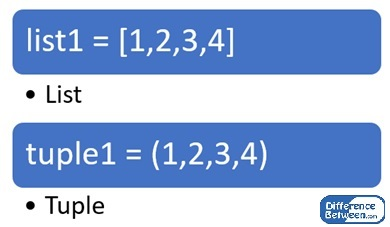
\includegraphics{Difference-Between-List-and-Tuple-fig-1-2.jpg}
\caption{At first glance list and tuples look very similar, but they are
not\ldots{}}
\end{figure}

Like lists, tuples are containers of any type of object. Unlike lists
though they are \emph{immutable} which means that once they have been
created the content cannot be changed (i.e.~no append, insert or delete
of the elements). Furthermore since they are immutable they can be used
as dictionary keys (lists cannot).

    \begin{Verbatim}[commandchars=\\\{\}]
{\color{incolor}In [{\color{incolor} }]:} \PY{n}{atuple} \PY{o}{=} \PY{p}{(}\PY{l+m+mi}{1}\PY{p}{,} \PY{l+m+mi}{2}\PY{p}{,} \PY{l+m+mi}{3}\PY{p}{)}
        \PY{n}{atuple}
\end{Verbatim}

    \begin{Verbatim}[commandchars=\\\{\}]
{\color{incolor}In [{\color{incolor} }]:} \PY{n+nb}{print} \PY{p}{(}\PY{l+s+s2}{\PYZdq{}}\PY{l+s+s2}{Length: }\PY{l+s+si}{\PYZob{}\PYZcb{}}\PY{l+s+s2}{\PYZdq{}}\PY{o}{.}\PY{n}{format}\PY{p}{(}\PY{n+nb}{len}\PY{p}{(}\PY{n}{atuple}\PY{p}{)}\PY{p}{)}\PY{p}{)}
        \PY{n+nb}{print} \PY{p}{(}\PY{l+s+s2}{\PYZdq{}}\PY{l+s+s2}{First element: }\PY{l+s+si}{\PYZob{}\PYZcb{}}\PY{l+s+s2}{\PYZdq{}}\PY{o}{.}\PY{n}{format}\PY{p}{(}\PY{n}{atuple}\PY{p}{[}\PY{l+m+mi}{0}\PY{p}{]}\PY{p}{)}\PY{p}{)}
        \PY{n+nb}{print} \PY{p}{(}\PY{l+s+s2}{\PYZdq{}}\PY{l+s+s2}{Last element: }\PY{l+s+si}{\PYZob{}\PYZcb{}}\PY{l+s+s2}{\PYZdq{}}\PY{o}{.}\PY{n}{format}\PY{p}{(}\PY{n}{atuple}\PY{p}{[}\PY{o}{\PYZhy{}}\PY{l+m+mi}{1}\PY{p}{]}\PY{p}{)}\PY{p}{)}
\end{Verbatim}

    \begin{Verbatim}[commandchars=\\\{\}]
{\color{incolor}In [{\color{incolor} }]:} \PY{n}{x}\PY{p}{,} \PY{n}{y}\PY{p}{,} \PY{n}{z} \PY{o}{=} \PY{p}{(}\PY{l+m+mi}{10}\PY{p}{,} \PY{l+m+mi}{5}\PY{p}{,} \PY{l+m+mi}{12}\PY{p}{)} \PY{c+c1}{\PYZsh{} this is called unpacking and it\PYZsq{}s another }
                              \PY{c+c1}{\PYZsh{} way to access tuple elements}
        \PY{n+nb}{print} \PY{p}{(}\PY{l+s+s2}{\PYZdq{}}\PY{l+s+s2}{coord: x=}\PY{l+s+si}{\PYZob{}\PYZcb{}}\PY{l+s+s2}{ y=}\PY{l+s+si}{\PYZob{}\PYZcb{}}\PY{l+s+s2}{ z=}\PY{l+s+si}{\PYZob{}\PYZcb{}}\PY{l+s+s2}{\PYZdq{}}\PY{o}{.}\PY{n}{format}\PY{p}{(}\PY{n}{x}\PY{p}{,} \PY{n}{y}\PY{p}{,} \PY{n}{z}\PY{p}{)}\PY{p}{)}
\end{Verbatim}

    \begin{Verbatim}[commandchars=\\\{\}]
{\color{incolor}In [{\color{incolor} }]:} \PY{n}{tuple2} \PY{o}{=} \PY{p}{(}\PY{l+m+mi}{1}\PY{p}{,}\PY{p}{)} \PY{c+c1}{\PYZsh{} this is tricky, don\PYZsq{}t forget the comma otherwise }
                      \PY{c+c1}{\PYZsh{} it won\PYZsq{}t be a tuple}
        \PY{n+nb}{print}\PY{p}{(}\PY{n+nb}{type}\PY{p}{(}\PY{n}{tuple2}\PY{p}{)}\PY{p}{)}
        \PY{n}{tuple2} \PY{o}{=} \PY{p}{(}\PY{l+m+mi}{1}\PY{p}{)}
        \PY{n+nb}{print}\PY{p}{(}\PY{n+nb}{type}\PY{p}{(}\PY{n}{tuple2}\PY{p}{)}\PY{p}{)}
\end{Verbatim}

    \begin{Verbatim}[commandchars=\\\{\}]
{\color{incolor}In [{\color{incolor} }]:} \PY{n}{tuple1} \PY{o}{=} \PY{p}{(}\PY{l+m+mi}{1}\PY{p}{,} \PY{l+m+mi}{2}\PY{p}{,} \PY{l+m+mi}{3}\PY{p}{)}
        \PY{n}{tuple2} \PY{o}{=} \PY{n}{tuple1} \PY{o}{+} \PY{p}{(}\PY{l+m+mi}{4}\PY{p}{,} \PY{l+m+mi}{5}\PY{p}{)} \PY{c+c1}{\PYZsh{} to add elements you need to create a new tuple}
        \PY{n}{tuple2} 
\end{Verbatim}

    \begin{Verbatim}[commandchars=\\\{\}]
{\color{incolor}In [{\color{incolor} }]:} \PY{c+c1}{\PYZsh{} as said they can be used as dictionary keys}
        \PY{n}{d} \PY{o}{=} \PY{p}{\PYZob{}}
        \PY{p}{(}\PY{l+s+s1}{\PYZsq{}}\PY{l+s+s1}{Finance}\PY{l+s+s1}{\PYZsq{}}\PY{p}{,} \PY{l+m+mi}{1}\PY{p}{)}\PY{p}{:} \PY{l+s+s1}{\PYZsq{}}\PY{l+s+s1}{Room 8}\PY{l+s+s1}{\PYZsq{}}\PY{p}{,}
        \PY{p}{(}\PY{l+s+s1}{\PYZsq{}}\PY{l+s+s1}{Finance}\PY{l+s+s1}{\PYZsq{}}\PY{p}{,} \PY{l+m+mi}{2}\PY{p}{)}\PY{p}{:} \PY{l+s+s1}{\PYZsq{}}\PY{l+s+s1}{Room 3}\PY{l+s+s1}{\PYZsq{}}\PY{p}{,}
        \PY{p}{(}\PY{l+s+s1}{\PYZsq{}}\PY{l+s+s1}{Math}\PY{l+s+s1}{\PYZsq{}}\PY{p}{,} \PY{l+m+mi}{1}\PY{p}{)}\PY{p}{:} \PY{l+s+s1}{\PYZsq{}}\PY{l+s+s1}{Room 6}\PY{l+s+s1}{\PYZsq{}}\PY{p}{,}
        \PY{p}{(}\PY{l+s+s1}{\PYZsq{}}\PY{l+s+s1}{Programming}\PY{l+s+s1}{\PYZsq{}}\PY{p}{,} \PY{l+m+mi}{1}\PY{p}{)}\PY{p}{:} \PY{l+s+s1}{\PYZsq{}}\PY{l+s+s1}{IT room}\PY{l+s+s1}{\PYZsq{}}
        \PY{p}{\PYZcb{}}
        \PY{n}{d}
\end{Verbatim}

    \hypertarget{dates}{%
\subsection{Dates}\label{dates}}

Dates are not usually included in a standard beginner Python tutorial,
however since they are pretty essential for finance we are going to
cover this topic. In Python the standard date class lives in the
\texttt{datetime} module. We are also going to import
\texttt{relativedelta} from the \texttt{dateutil} module, which allows
us to add/subtract days/months/years to dates.

    \begin{Verbatim}[commandchars=\\\{\}]
{\color{incolor}In [{\color{incolor} }]:} \PY{k+kn}{from} \PY{n+nn}{datetime} \PY{k}{import} \PY{n}{date}
        \PY{k+kn}{from} \PY{n+nn}{dateutil}\PY{n+nn}{.}\PY{n+nn}{relativedelta} \PY{k}{import} \PY{n}{relativedelta}
\end{Verbatim}

    \begin{Verbatim}[commandchars=\\\{\}]
{\color{incolor}In [{\color{incolor} }]:} \PY{n}{date}\PY{o}{.}\PY{n}{today}\PY{p}{(}\PY{p}{)}
\end{Verbatim}

    \begin{Verbatim}[commandchars=\\\{\}]
{\color{incolor}In [{\color{incolor} }]:} \PY{n}{date}\PY{o}{.}\PY{n}{today}\PY{p}{(}\PY{p}{)} \PY{o}{+} \PY{n}{relativedelta}\PY{p}{(}\PY{n}{months}\PY{o}{=}\PY{l+m+mi}{2}\PY{p}{)}
\end{Verbatim}

    \begin{Verbatim}[commandchars=\\\{\}]
{\color{incolor}In [{\color{incolor} }]:} \PY{n}{date}\PY{o}{.}\PY{n}{today}\PY{p}{(}\PY{p}{)} \PY{o}{\PYZhy{}} \PY{n}{relativedelta}\PY{p}{(}\PY{n}{days}\PY{o}{=}\PY{l+m+mi}{3}\PY{p}{)}
\end{Verbatim}

    \begin{Verbatim}[commandchars=\\\{\}]
{\color{incolor}In [{\color{incolor} }]:} \PY{n}{one\PYZus{}day} \PY{o}{=} \PY{n}{relativedelta}\PY{p}{(}\PY{n}{days}\PY{o}{=}\PY{l+m+mi}{1}\PY{p}{)}
        \PY{n}{date}\PY{o}{.}\PY{n}{today}\PY{p}{(}\PY{p}{)} \PY{o}{\PYZhy{}} \PY{l+m+mi}{3} \PY{o}{*} \PY{n}{one\PYZus{}day}
\end{Verbatim}

    \begin{Verbatim}[commandchars=\\\{\}]
{\color{incolor}In [{\color{incolor} }]:} \PY{n}{date1} \PY{o}{=} \PY{n}{date}\PY{p}{(}\PY{l+m+mi}{2019}\PY{p}{,} \PY{l+m+mi}{7}\PY{p}{,} \PY{l+m+mi}{2}\PY{p}{)}
        \PY{n}{date2} \PY{o}{=} \PY{n}{date}\PY{p}{(}\PY{l+m+mi}{2019}\PY{p}{,} \PY{l+m+mi}{8}\PY{p}{,} \PY{l+m+mi}{16}\PY{p}{)}
        \PY{p}{(}\PY{n}{date2} \PY{o}{\PYZhy{}} \PY{n}{date1}\PY{p}{)}\PY{o}{.}\PY{n}{days}
\end{Verbatim}

    \begin{Verbatim}[commandchars=\\\{\}]
{\color{incolor}In [{\color{incolor} }]:} \PY{n+nb}{print} \PY{p}{(}\PY{n+nb}{type}\PY{p}{(}\PY{n}{date1}\PY{p}{)}\PY{p}{)}
        \PY{n+nb}{print} \PY{p}{(}\PY{n}{date1}\PY{p}{)}
        \PY{n}{date1} \PY{o}{=} \PY{n+nb}{str}\PY{p}{(}\PY{n}{date1}\PY{p}{)} \PY{c+c1}{\PYZsh{} converts (or \PYZsq{}cast\PYZsq{}) a date to a string}
        \PY{n+nb}{print} \PY{p}{(}\PY{n}{date1}\PY{p}{)}
        \PY{n+nb}{print} \PY{p}{(}\PY{n+nb}{type}\PY{p}{(}\PY{n}{date1}\PY{p}{)}\PY{p}{)}
\end{Verbatim}

    \begin{Verbatim}[commandchars=\\\{\}]
{\color{incolor}In [{\color{incolor} }]:} \PY{n}{date1} \PY{o}{=} \PY{n}{date}\PY{p}{(}\PY{l+m+mi}{2019}\PY{p}{,} \PY{l+m+mi}{7}\PY{p}{,} \PY{l+m+mi}{2}\PY{p}{)}
        \PY{n}{date1}\PY{o}{.}\PY{n}{strftime}\PY{p}{(}\PY{l+s+s2}{\PYZdq{}}\PY{l+s+s2}{\PYZpc{}}\PY{l+s+s2}{Y\PYZhy{}}\PY{l+s+s2}{\PYZpc{}}\PY{l+s+s2}{b\PYZhy{}}\PY{l+s+si}{\PYZpc{}d}\PY{l+s+s2}{ (}\PY{l+s+si}{\PYZpc{}a}\PY{l+s+s2}{)}\PY{l+s+s2}{\PYZdq{}}\PY{p}{)} \PY{c+c1}{\PYZsh{} dates can formatted in many ways}
                                        \PY{c+c1}{\PYZsh{} check the docs for more details}
\end{Verbatim}

    \begin{Verbatim}[commandchars=\\\{\}]
{\color{incolor}In [{\color{incolor} }]:} \PY{c+c1}{\PYZsh{} a string can be convered to dates too}
        \PY{k+kn}{from} \PY{n+nn}{datetime} \PY{k}{import} \PY{n}{datetime}
        \PY{n}{datetime}\PY{o}{.}\PY{n}{strptime}\PY{p}{(}\PY{l+s+s1}{\PYZsq{}}\PY{l+s+s1}{25 Aug 2019}\PY{l+s+s1}{\PYZsq{}}\PY{p}{,} \PY{l+s+s2}{\PYZdq{}}\PY{l+s+si}{\PYZpc{}d}\PY{l+s+s2}{ }\PY{l+s+s2}{\PYZpc{}}\PY{l+s+s2}{b }\PY{l+s+s2}{\PYZpc{}}\PY{l+s+s2}{Y}\PY{l+s+s2}{\PYZdq{}}\PY{p}{)}\PY{o}{.}\PY{n}{date}\PY{p}{(}\PY{p}{)}
\end{Verbatim}

    \begin{Verbatim}[commandchars=\\\{\}]
{\color{incolor}In [{\color{incolor} }]:} \PY{n}{date1}\PY{o}{.}\PY{n}{weekday}\PY{p}{(}\PY{p}{)} \PY{c+c1}{\PYZsh{} 0 = monday, ..., 6 = sunday}
\end{Verbatim}

    \hypertarget{exercise-2.1}{%
\subsubsection{Exercise 2.1}\label{exercise-2.1}}

Write code in the notebook to:

\begin{itemize}
\tightlist
\item
  print the day of the week of your birthday
\item
  print the weekday of your birthdays for the next 120 years
\end{itemize}

(expected output: Sun 1 Mon 2 Sun \ldots{} 119 Thu 120 Sun)

    \hypertarget{functions}{%
\subsection{Functions}\label{functions}}

A function is a block of organized, reusable code that is used to
perform a single action. Functions provide better modularity for your
application and high degree of code reusing.

    \begin{Verbatim}[commandchars=\\\{\}]
{\color{incolor}In [{\color{incolor} }]:} \PY{c+c1}{\PYZsh{} sum up all the integers between 1 and n }
        \PY{k}{def} \PY{n+nf}{my\PYZus{}function}\PY{p}{(}\PY{n}{n}\PY{p}{)}\PY{p}{:} \PY{c+c1}{\PYZsh{} this function take one input only (n)}
            \PY{n}{x} \PY{o}{=} \PY{l+m+mi}{0}
            \PY{k}{for} \PY{n}{i} \PY{o+ow}{in} \PY{n+nb}{range}\PY{p}{(}\PY{l+m+mi}{1}\PY{p}{,} \PY{n}{n}\PY{o}{+}\PY{l+m+mi}{1}\PY{p}{)}\PY{p}{:}
                \PY{n}{x} \PY{o}{+}\PY{o}{=} \PY{n}{i}
            \PY{k}{return} \PY{n}{x} \PY{c+c1}{\PYZsh{} the function returns a number}
\end{Verbatim}

    \begin{Verbatim}[commandchars=\\\{\}]
{\color{incolor}In [{\color{incolor} }]:} \PY{n}{my\PYZus{}function}\PY{p}{(}\PY{l+m+mi}{5}\PY{p}{)} \PY{c+c1}{\PYZsh{} 5 + 4 + 3 + 2 + 1}
\end{Verbatim}

    To be clear functions can return any kind of objects (numbers, strings,
lists, complex objects\ldots{}) but it is not mandatory, so you can
write a function \textbf{without} a \texttt{return} statement.

\begin{Shaded}
\begin{Highlighting}[]
\KeywordTok{def}\NormalTok{ printing(mystring):}
    \BuiltInTok{print}\NormalTok{ (myString)}
\end{Highlighting}
\end{Shaded}

In addition the syntax of the \texttt{return} is different from
\texttt{Visual\ Basic}, the returned object doesn't have to have the
same name as the function.

    \begin{Verbatim}[commandchars=\\\{\}]
{\color{incolor}In [{\color{incolor} }]:} \PY{k}{def} \PY{n+nf}{my\PYZus{}function\PYZus{}2}\PY{p}{(}\PY{n}{n}\PY{p}{,} \PY{n}{x}\PY{p}{)}\PY{p}{:} 
            \PY{k}{return} \PY{l+s+s2}{\PYZdq{}}\PY{l+s+s2}{The result is : }\PY{l+s+si}{\PYZob{}\PYZcb{}}\PY{l+s+s2}{\PYZdq{}}\PY{o}{.}\PY{n}{format}\PY{p}{(}\PY{n+nb}{str}\PY{p}{(}\PY{n}{my\PYZus{}function}\PY{p}{(}\PY{n}{n}\PY{p}{)}\PY{o}{*}\PY{n}{x}\PY{p}{)}\PY{p}{)}
        \PY{c+c1}{\PYZsh{} returns x * result of my\PYZus{}function(n)}
        \PY{c+c1}{\PYZsh{} so function of function}
\end{Verbatim}

    \begin{Verbatim}[commandchars=\\\{\}]
{\color{incolor}In [{\color{incolor} }]:} \PY{n}{my\PYZus{}function\PYZus{}2}\PY{p}{(}\PY{l+m+mi}{5}\PY{p}{,} \PY{l+m+mi}{10}\PY{p}{)}
\end{Verbatim}

    Functions can also call themselves too (i.e \emph{recursion}). In the
next example we write a function that computes the factorial exploiting
the following relationship:

\[ \begin{split}n! = n \times (n-1)! & \;\; (\forall n \gt 1) \\
    n! = 1 & \;\; (\forall n \le 1)
    \end{split}
\]

    \begin{Verbatim}[commandchars=\\\{\}]
{\color{incolor}In [{\color{incolor} }]:} \PY{k}{def} \PY{n+nf}{factorial}\PY{p}{(}\PY{n}{n}\PY{p}{)}\PY{p}{:}
            \PY{k}{if} \PY{n}{n} \PY{o}{\PYZlt{}}\PY{o}{=} \PY{l+m+mi}{1}\PY{p}{:}
                \PY{k}{return} \PY{l+m+mi}{1}
            \PY{k}{else}\PY{p}{:}
                \PY{k}{return} \PY{n}{n} \PY{o}{*} \PY{n}{factorial}\PY{p}{(}\PY{n}{n}\PY{o}{\PYZhy{}}\PY{l+m+mi}{1}\PY{p}{)}
\end{Verbatim}

    \begin{Verbatim}[commandchars=\\\{\}]
{\color{incolor}In [{\color{incolor} }]:} \PY{n}{factorial}\PY{p}{(}\PY{l+m+mi}{10}\PY{p}{)}
\end{Verbatim}

    Functions can accept and return any values and arguments can have
default values.

    \begin{Verbatim}[commandchars=\\\{\}]
{\color{incolor}In [{\color{incolor} }]:} \PY{k}{def} \PY{n+nf}{powers}\PY{p}{(}\PY{n}{xs}\PY{p}{,} \PY{n}{n} \PY{o}{=} \PY{l+m+mi}{2}\PY{p}{,} \PY{n}{c} \PY{o}{=} \PY{l+m+mi}{0}\PY{p}{)}\PY{p}{:}
            \PY{k}{return} \PY{p}{\PYZob{}}\PY{n}{x}\PY{p}{:} \PY{n}{x}\PY{o}{*}\PY{o}{*}\PY{n}{n}\PY{o}{+}\PY{n}{c} \PY{k}{for} \PY{n}{x} \PY{o+ow}{in} \PY{n}{xs}\PY{p}{\PYZcb{}}
\end{Verbatim}

    \begin{Verbatim}[commandchars=\\\{\}]
{\color{incolor}In [{\color{incolor} }]:} \PY{n}{powers}\PY{p}{(}\PY{p}{[}\PY{l+m+mi}{5}\PY{p}{,} \PY{l+m+mi}{11}\PY{p}{,} \PY{l+m+mi}{6}\PY{p}{]}\PY{p}{)} \PY{c+c1}{\PYZsh{} calling powers like this results in 25, 121 and 36}
                           \PY{c+c1}{\PYZsh{} since n = 2 and c = 0 by default if not specified}
\end{Verbatim}

    A nice feature of Pyhton functions is that we can associate an help
message to them so that we can easily check what a function is for by
simply asking

\begin{Shaded}
\begin{Highlighting}[]
\BuiltInTok{help}\NormalTok{(function_name)}
\end{Highlighting}
\end{Shaded}

    \begin{Verbatim}[commandchars=\\\{\}]
{\color{incolor}In [{\color{incolor} }]:} \PY{k}{def} \PY{n+nf}{powers}\PY{p}{(}\PY{n}{xs}\PY{p}{,} \PY{n}{n}\PY{o}{=}\PY{l+m+mi}{2}\PY{p}{,} \PY{n}{c}\PY{o}{=}\PY{l+m+mi}{0}\PY{p}{)}\PY{p}{:}
            \PY{l+s+sd}{\PYZsq{}\PYZsq{}\PYZsq{} a shifted power function example in lesson 2}
        \PY{l+s+sd}{    }
        \PY{l+s+sd}{    x ** n + c}
        \PY{l+s+sd}{    }
        \PY{l+s+sd}{    \PYZsq{}\PYZsq{}\PYZsq{}}
            \PY{k}{return} \PY{p}{\PYZob{}}\PY{n}{x}\PY{p}{:} \PY{n}{x} \PY{o}{*}\PY{o}{*} \PY{n}{n} \PY{o}{+} \PY{n}{c} \PY{k}{for} \PY{n}{x} \PY{o+ow}{in} \PY{n}{xs}\PY{p}{\PYZcb{}}
\end{Verbatim}

    \begin{Verbatim}[commandchars=\\\{\}]
{\color{incolor}In [{\color{incolor} }]:} \PY{n}{help}\PY{p}{(}\PY{n}{powers}\PY{p}{)}
\end{Verbatim}

    \hypertarget{advanced---variable-scope}{%
\subsection{Advanced - Variable scope}\label{advanced---variable-scope}}

Not all variables are accessible from all parts of our program, and not
all variables exist for the same amount of time. We call the part of a
program where a variable is accessible its scope.

A variable which is defined in the main body of a file is called a
global variable. It will be visible throughout the file, and also inside
any file which imports that file. Global variables can have unintended
consequences because of their wide-ranging effects -- that is why we
should almost never use them (usually they are represented by an
uppercase name). Only objects which are intended to be used globally,
like functions and classes, should be put in the global namespace.

Global variables can be accessed directly inside a function but cannot
be modified. To modify them you have to use the keyword \texttt{global}:

    \begin{Verbatim}[commandchars=\\\{\}]
{\color{incolor}In [{\color{incolor} }]:} \PY{n}{AGLOBALPARAM} \PY{o}{=} \PY{l+m+mi}{10}
        
        \PY{c+c1}{\PYZsh{} Here you just use AGLOBALPARAM value, but do not modify it}
        \PY{c+c1}{\PYZsh{} param is just a copy of AGLOBALPARAM}
        \PY{k}{def} \PY{n+nf}{multiplyParam}\PY{p}{(}\PY{n}{param}\PY{p}{)}\PY{p}{:} 
            \PY{n}{param} \PY{o}{=} \PY{n}{param} \PY{o}{*} \PY{l+m+mi}{10}
            \PY{k}{return} \PY{p}{(}\PY{n}{param}\PY{p}{)}
        
        \PY{c+c1}{\PYZsh{} Here you actually use AGLOBALPARAM}
        \PY{c+c1}{\PYZsh{} you modify it directly}
        \PY{k}{def} \PY{n+nf}{divideParam}\PY{p}{(}\PY{p}{)}\PY{p}{:}
            \PY{k}{global} \PY{n}{AGLOBALPARAM}
            \PY{n}{AGLOBALPARAM} \PY{o}{=} \PY{n}{AGLOBALPARAM} \PY{o}{/} \PY{l+m+mi}{10}
            \PY{k}{return} \PY{p}{(}\PY{n}{AGLOBALPARAM}\PY{p}{)}
            
        \PY{c+c1}{\PYZsh{} Here you try to use AGLOBALPARAM but gives you an error}
        \PY{c+c1}{\PYZsh{} it is not accessible !}
        \PY{k}{def} \PY{n+nf}{sumParam}\PY{p}{(}\PY{p}{)}\PY{p}{:}
            \PY{n}{AGLOBALPARAM} \PY{o}{=} \PY{n}{AGLOBALPARAM} \PY{o}{+} \PY{l+m+mi}{10}
            \PY{k}{return} \PY{p}{(}\PY{n}{AGLOBALPARAM} \PY{o}{+} \PY{n}{x}\PY{p}{)}
        
        \PY{n+nb}{print} \PY{p}{(}\PY{l+s+s2}{\PYZdq{}}\PY{l+s+s2}{AGLOBALPARAM is }\PY{l+s+si}{\PYZob{}\PYZcb{}}\PY{l+s+s2}{ to start.}\PY{l+s+s2}{\PYZdq{}}\PY{o}{.}\PY{n}{format}\PY{p}{(}\PY{n}{AGLOBALPARAM}\PY{p}{)}\PY{p}{)}
        \PY{n+nb}{print} \PY{p}{(}\PY{l+s+s2}{\PYZdq{}}\PY{l+s+s2}{Let}\PY{l+s+s2}{\PYZsq{}}\PY{l+s+s2}{s multiply it by 10.}\PY{l+s+s2}{\PYZdq{}}\PY{p}{)}
        \PY{n}{multiplyParam}\PY{p}{(}\PY{n}{AGLOBALPARAM}\PY{p}{)}
        \PY{n+nb}{print} \PY{p}{(}\PY{l+s+s2}{\PYZdq{}}\PY{l+s+s2}{AGLOBALPARAM is still }\PY{l+s+si}{\PYZob{}\PYZcb{}}\PY{l+s+s2}{\PYZdq{}}\PY{o}{.}\PY{n}{format}\PY{p}{(}\PY{n}{AGLOBALPARAM}\PY{p}{)}\PY{p}{)}
        \PY{n+nb}{print} \PY{p}{(}\PY{l+s+s2}{\PYZdq{}}\PY{l+s+s2}{Let}\PY{l+s+s2}{\PYZsq{}}\PY{l+s+s2}{s divide it by 10}\PY{l+s+s2}{\PYZdq{}}\PY{p}{)}
        \PY{n}{divideParam}\PY{p}{(}\PY{p}{)}
        \PY{n+nb}{print} \PY{p}{(}\PY{l+s+s2}{\PYZdq{}}\PY{l+s+s2}{Now AGLOBALPARAM is }\PY{l+s+si}{\PYZob{}\PYZcb{}}\PY{l+s+s2}{\PYZdq{}}\PY{o}{.}\PY{n}{format}\PY{p}{(}\PY{n}{AGLOBALPARAM}\PY{p}{)}\PY{p}{)}
        \PY{n+nb}{print} \PY{p}{(}\PY{l+s+s2}{\PYZdq{}}\PY{l+s+s2}{Let}\PY{l+s+s2}{\PYZsq{}}\PY{l+s+s2}{s sum it to 10}\PY{l+s+s2}{\PYZdq{}}\PY{p}{)}
        \PY{n}{sumParam}\PY{p}{(}\PY{p}{)}
\end{Verbatim}

    A variable which is defined inside a function is local to that function.
It is accessible from the point at which it is defined until the end of
the function (e.g.~the parameter names in the function definition behave
like local variables).

    \begin{Verbatim}[commandchars=\\\{\}]
{\color{incolor}In [{\color{incolor} }]:} \PY{c+c1}{\PYZsh{} functions are not evaluated if not called}
        \PY{k}{def} \PY{n+nf}{test\PYZus{}scope}\PY{p}{(}\PY{n}{max\PYZus{}val}\PY{p}{)}\PY{p}{:}
            \PY{k}{for} \PY{n}{i} \PY{o+ow}{in} \PY{n+nb}{range}\PY{p}{(}\PY{n}{max\PYZus{}val}\PY{p}{)}\PY{p}{:}
                \PY{n+nb}{print} \PY{p}{(}\PY{n}{i}\PY{p}{)}
            \PY{n+nb}{print} \PY{p}{(}\PY{l+s+s2}{\PYZdq{}}\PY{l+s+s2}{max\PYZus{}val in }\PY{l+s+s2}{\PYZsq{}}\PY{l+s+s2}{test\PYZus{}scope}\PY{l+s+s2}{\PYZsq{}}\PY{l+s+s2}{ function is }\PY{l+s+si}{\PYZob{}\PYZcb{}}\PY{l+s+s2}{\PYZdq{}}\PY{o}{.}\PY{n}{format}\PY{p}{(}\PY{n}{max\PYZus{}val}\PY{p}{)}\PY{p}{)}
            
        \PY{c+c1}{\PYZsh{} the Python interpreter starts evaluating the code from here    }
        \PY{n}{max\PYZus{}val} \PY{o}{=} \PY{l+m+mi}{10}
        \PY{n}{test\PYZus{}scope}\PY{p}{(}\PY{l+m+mi}{5}\PY{p}{)}
        \PY{n+nb}{print} \PY{p}{(}\PY{l+s+s2}{\PYZdq{}}\PY{l+s+s2}{max\PYZus{}val in global scope is }\PY{l+s+si}{\PYZob{}\PYZcb{}}\PY{l+s+s2}{\PYZdq{}}\PY{o}{.}\PY{n}{format}\PY{p}{(}\PY{n}{max\PYZus{}val}\PY{p}{)}\PY{p}{)}
        \PY{n+nb}{print} \PY{p}{(}\PY{n}{i}\PY{p}{)}
\end{Verbatim}

    \hypertarget{exercises-for-next-week}{%
\subsection{Exercises for next week}\label{exercises-for-next-week}}

\hypertarget{exercise-2.2}{%
\subsubsection{Exercise 2.2}\label{exercise-2.2}}

Write code which, given the following list

\begin{Shaded}
\begin{Highlighting}[]
\NormalTok{input_list }\OperatorTok{=}\NormalTok{ [}\DecValTok{3}\NormalTok{, }\DecValTok{5}\NormalTok{, }\DecValTok{2}\NormalTok{, }\DecValTok{1}\NormalTok{, }\DecValTok{13}\NormalTok{, }\DecValTok{5}\NormalTok{, }\DecValTok{5}\NormalTok{, }\DecValTok{1}\NormalTok{, }\DecValTok{3}\NormalTok{, }\DecValTok{4}\NormalTok{]}
\end{Highlighting}
\end{Shaded}

prints out the indices of every occurrence of

\begin{Shaded}
\begin{Highlighting}[]
\NormalTok{y }\OperatorTok{=} \DecValTok{5}
\end{Highlighting}
\end{Shaded}

\hypertarget{exercise-2.3}{%
\subsubsection{Exercise 2.3}\label{exercise-2.3}}

Given the following variables

\begin{Shaded}
\begin{Highlighting}[]
\NormalTok{S_t }\OperatorTok{=} \FloatTok{800.0} \CommentTok{# spot price of the underlying<br>}
\NormalTok{K }\OperatorTok{=} \FloatTok{600.0}   \CommentTok{# strike price<br>}
\NormalTok{vol }\OperatorTok{=} \FloatTok{0.25}  \CommentTok{# volatility<br>}
\NormalTok{r }\OperatorTok{=} \FloatTok{0.01}    \CommentTok{# interest rate<br>}
\NormalTok{ttm }\OperatorTok{=} \FloatTok{0.5}   \CommentTok{# time to maturity, in years<br>}
\end{Highlighting}
\end{Shaded}

write out the Black Scholes formula and save the value of a call in a
variable named `call\_price' and the value of a put in a variable named
`put\_price'

\hypertarget{exercise-2.4}{%
\subsubsection{Exercise 2.4}\label{exercise-2.4}}

Given the following dictionary mapping currencies to 2-year zero coupon
bond prices, build another dictionary mapping the same currencies to the
corresponding annualized interest rates.

\begin{Shaded}
\begin{Highlighting}[]
\NormalTok{d }\OperatorTok{=}\NormalTok{ \{}
\StringTok{'EUR'}\NormalTok{: }\FloatTok{0.98}\NormalTok{,}
\StringTok{'CHF'}\NormalTok{: }\FloatTok{1.005}\NormalTok{,}
\StringTok{'USD'}\NormalTok{: }\FloatTok{0.985}\NormalTok{,}
\StringTok{'GBP'}\NormalTok{: }\FloatTok{0.97}
\NormalTok{\}}
\end{Highlighting}
\end{Shaded}

\hypertarget{exercise-2.5}{%
\subsubsection{Exercise 2.5}\label{exercise-2.5}}

Build again dates as in Exercise 2.1 (i.e.~the weekday of your birthdays
for the next 120 years) and count how many of your birthdays is a
Monday, Tuesday, \ldots{} , Sunday until 120 years of age. Print out the
result using a dictionary. (expected output somenthing like:
\texttt{python\ \{6:\ 10,\ 0:\ 10,\ 2:\ 9,\ 3:\ 10,\ 4:\ 10,\ 5:\ 10,\ 1:\ 9\}})


    % Add a bibliography block to the postdoc
    
    
    
    \end{document}
